\documentclass[a4paper,12pt]{report}

\usepackage[portuguese]{babel}
\usepackage{indentfirst}
\usepackage[T1]{fontenc}
\usepackage[utf8]{inputenc}
\usepackage{csquotes}
\usepackage{array}
\usepackage[font={footnotesize,it}]{caption}
\usepackage{graphicx} 
\usepackage{float}
\usepackage{color, colortbl}
\usepackage{titlesec}
\usepackage{longtable}
\usepackage{pdfpages} 
\usepackage{tabularx}
\usepackage[hidelinks]{hyperref}
%\usepackage{lmodern} 

\graphicspath{ {../plots/bivariateAnalysis}{../plots/dataUnderstanding}{../plots/processing}}


\setlength{\parskip}{\baselineskip}
%\usepackage[top=2.5cm, bottom=2.5cm, left=3cm, right=2.5cm]{geometry}

%--------------------------------------------------------------
\begin{document}

	\begin{titlepage}
		
		\begin{center}
		
		% \begin{figure}[H]
		% \begin{center}
		% 	\includegraphics[scale=0.45]{utad_logo}	
		% \end{center}
		% \label{fig:logoUTAD}	
		% \end{figure}
		
		
		\vspace{3cm}
		\huge
		\textbf{Data Mining Project}
		
		%\vspace{0.5cm}
		\Large
		Work Summary\\
		
		
		\vspace{2.5cm}
		\large
		Autor\\

		
		\vspace{3cm}
		Machine Learning\\
		Master's degree in Informatics and Computing Engineering \\
		
		\vspace{2cm}		
		Porto, 2021
		
		\end{center}
	\end{titlepage}	
	
	
%--------------------------------------------------------------
	
	\pagenumbering{roman}
	
	\begin{abstract}
	
	\end{abstract}	
	
	
	\newpage
	\tableofcontents
	
	\pagenumbering{arabic}
	\newpage	
	
%	\begin{figure}[H]
%	\begin{center}
%	\includegraphics[scale=0.85]{equacao}	
%	\end{center}
%	\caption{Equação do problema.}
%	\label{fig:equacao}
%	\end{figure}



%	\begin{table}[H]
%	\begin{center}
%	\begin{tabular}{ |c|c| } 
%	 \hline
%	 Teste & Melhor Solução\\ 
%	 \hline
% 	 \hline
% 	 1 & 0.00082033\\
% 	 \hline 
%	\end{tabular}
%	\end{center}
%	\caption{Resultados de 15 testes com a implementação do \textit{Simulated Annealing}.}
%	\label{tab:tabela_SA}
%	\end{table}
	
%--------------------------------------------------------------	
\chapter{Business Understanding}

\begin{itemize}
    \item Analysis of requirements with the end user.
    \item Definition of business goals.
    \item Translation of business goals into data mining goals.
\end{itemize}




%--------------------------------------------------------------	
\chapter{Data Understanding}

\begin{itemize}
    \item Diversity of statistical methods.
	\item Complexity of statistical methods.
	\item Interpretation of results of statistical methods.
	\item Knowledge extraction from results of statistical methods.
	\item Diversity of plots.
	\item Complexity of plots.
	\item Presentation.
	\item Interpretation of plots.
	\item Visual knowledge extraction.
\end{itemize}

	\section{Plots - Data Understanding}

		Looking at this plot, we can observe that most of the unsuccessful loans are usually located on the left part of the chart, which means that people with low balances on their accounts are prone to fail loan payments.

		\begin{figure}[H]
		\begin{center}
		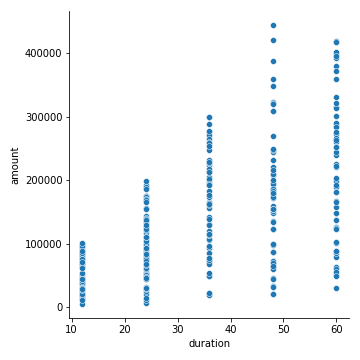
\includegraphics[scale=0.40]{ammount_duration_scatterPlot}	
		\end{center}
		\caption{Plot}
		\label{fig:ammount_duration_scatterPlot}
		\end{figure}

		As we can see in this plot, higher duration loans result typically in higher amounts.

		\begin{figure}[H]
		\begin{center}
		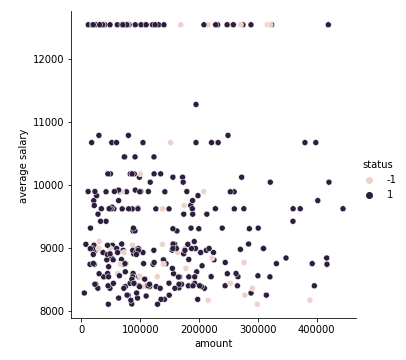
\includegraphics[scale=0.40]{avgSalary_ammount}	
		\end{center}
		\caption{Plot}
		\label{fig:avgSalary_ammount}
		\end{figure}

		\begin{figure}[H]
		\begin{center}
		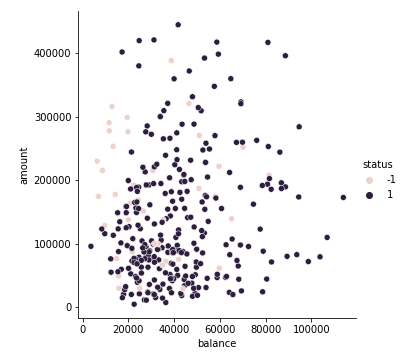
\includegraphics[scale=0.40]{balance_ammount_scatterPlot}	
		\end{center}
		\caption{Plot}
		\label{fig:balance_ammount_scatterPlot}
		\end{figure}


	\section{Plots - Processing}

		\begin{figure}[H]
		\begin{center}
		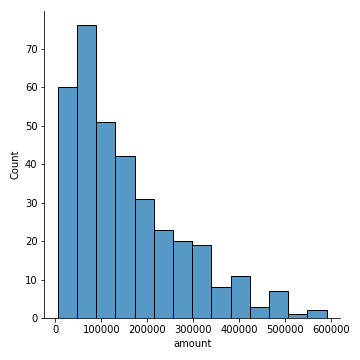
\includegraphics[scale=0.40]{amount_barChart}	
		\end{center}
		\caption{Plot.}
		\label{fig:amount_barChart}
		\end{figure}

		\begin{figure}[H]
		\begin{center}
		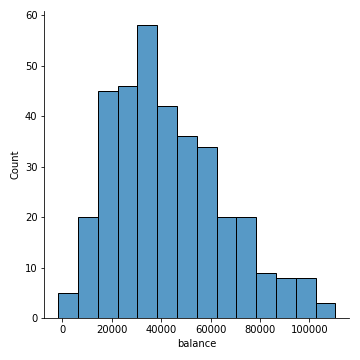
\includegraphics[scale=0.40]{balance_barChart}	
		\end{center}
		\caption{Plot.}
		\label{fig:balance_barChart}
		\end{figure}

		\begin{figure}[H]
		\begin{center}
		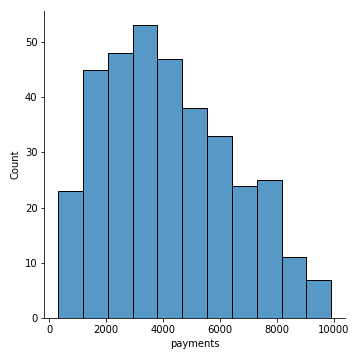
\includegraphics[scale=0.40]{payments_barChart}	
		\end{center}
		\caption{Plot.}
		\label{fig:payments_barChart}
		\end{figure}

		\begin{figure}[H]
		\begin{center}
		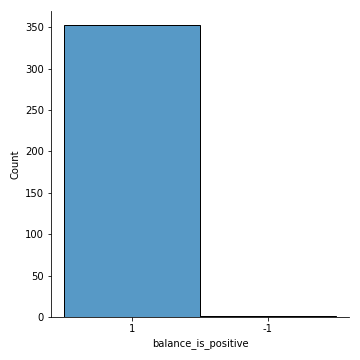
\includegraphics[scale=0.40]{positiveBalance_barChart}	
		\end{center}
		\caption{Plot.}
		\label{fig:positiveBalance_barChart}
		\end{figure}



%--------------------------------------------------------------	
\chapter{Data Processing}

\begin{itemize}
    \item Data integration.
    \item Assessment of dimensions of data quality.
    \item Cleaning redundancy.
    \item Cleaning missing data.
    \item Cleaning outliers.
    \item Data transformation for compatibility with algorithms.
    \item Feature engineering from tabular data.
    \item Sampling for domain-specific purposes.
    \item Sampling for development.
    \item Imbalanced data.
    \item Feature selection.
\end{itemize}


%--------------------------------------------------------------	
\chapter{Descriptive}

\begin{itemize}
    \item Diversity of algorithms.
    \item Parameter tunning.
    \item Understanding algorithm behaviour.
    \item Performance measure.
    \item Correct interpretation of performance measures.
    \item Comparative analysis of results.
    \item Model improvement.
    \item Analysis of resuls.
	\item Diversity of tasks.
	\item Diversity of algorithms.
\end{itemize}


%--------------------------------------------------------------	
\chapter{Predictive}

\begin{itemize}
    \item Parameter tunning.
	\item Undertanding algorithm behavior.
	\item Performance estimation: training vs test.
	\item Performance estimation: other factors (time, ...).
	\item Performance estimation: performance measure.
	\item Performance estimation: correct interpretation of performance measures.
	\item Performance estimation: analysis of results.
	\item Model improvement.
	\item Feature importance.
	\item Analysis of "white-box" models.
\end{itemize}
	


%--------------------------------------------------------------	
\chapter{Project}

\begin{itemize}
    \item Management methodology.
	\item Management plan.
	\item Project management tools.
	\item Collaboration tools.
\end{itemize}


	We are using Github for version control and collaboration. We regularly do pair programming using Visual Studio Code live sharing feature. 


%--------------------------------------------------------------	
\chapter{Tools}

\begin{itemize}
    \item Analytics.
	\item Database.
	\item Other tools (data cleaning, visualization).
\end{itemize}



%--------------------------------------------------------------	
\chapter{Presentation}

\begin{itemize}
    \item Quality of layout.
	\item Quality of content in slides.
	\item Delivery.
	\item Use of time. 
\end{itemize}


\end{document}